\documentclass{beamer}

\usetheme{Madrid}
\usecolortheme{default}
\usepackage{graphicx}
\usepackage{transparent}
\usepackage{hyperref}
\usepackage{graphicx}

\usebackgroundtemplate{%
  \parbox[c][\paperheight][c]{\paperwidth}{%
    \centering
    \transparent{0.15}
    
\includegraphics[width=6cm,height=\paperheight,keepaspectratio]{iitr.png}%
  }%
}
% \usebackgroundtemplate{%
%   \centering
%   \transparent{0.15} % 0 = invisible, 1 = fully visible
%   
\includegraphics[width=5cm,height=\paperheight,keepaspectratio]{iitr.png}
% }


\title{Digital Arrest Scam}
\subtitle{Problem, Impact, and Future Mitigation}
\author{Technical Communication}
\institute{Group 4}
\date{\today}

% \titlegraphic{
%   
\includegraphics[width=1.5cm]{iitr.png}
% }

\begin{document}

% Custom Title Slide
{
\usebackgroundtemplate{}
\begin{frame}[plain]
  \centering

  \vspace{0.5cm}
  
\includegraphics[width=3cm]{iitr.png}

  \vspace{0.6cm}
  {\LARGE \textbf{Digital Arrest Scam} \par}

  \vspace{0.3cm}
  {\large Problem, Impact and Future Mitigation \par}

  \vspace{0.6cm}
  {\normalsize Technical Communication \par}
  {\normalsize Group 4 \par}

  \vfill
  {\small \today}
\end{frame}
}


% Slide 1: Problem and Relevance
\begin{frame}{Digital Arrest: Problem and Relevance}

\textbf{What is Digital Arrest?}
\begin{itemize}
  \item A cyber fraud technique where scammers impersonate police, courts, or cybercrime officials
  \item False accusation of crimes are done using fake identity documents including forged FIRs, official IDs and warrants
  \item Victims are intimidated using threats of criminal charges and arrests
  \item Money is extorted through digital payments and cryptocurrency
\end{itemize}

\vspace{0.3cm}

\textbf{Why It’s Relevant Today}
\begin{itemize}
  \item Rapid digitalization of services and payment systems
  \item Increased risk of deception with advent of AI and deepfake tools
  \item Lack of public awareness about official legal and arrest procedures
\end{itemize}

\end{frame}

\begin{frame}{Social and Economic Impacts}

% ---------- Scale of the Problem with Graph ----------
\begin{columns}

% Left: Scale of the Problem text
\begin{column}{0.6\textwidth}
\textbf{Scale of the Problem}
\begin{itemize}
  \item In 2024, 123672 cases of digital arrest were reported in India
  \item A total of Rs. 1935.51 Cr were defrauded in 2024, as per GoI
\end{itemize}
\end{column}

% Right: Graph (Top Right)
\begin{column}{0.4\textwidth}
\centering
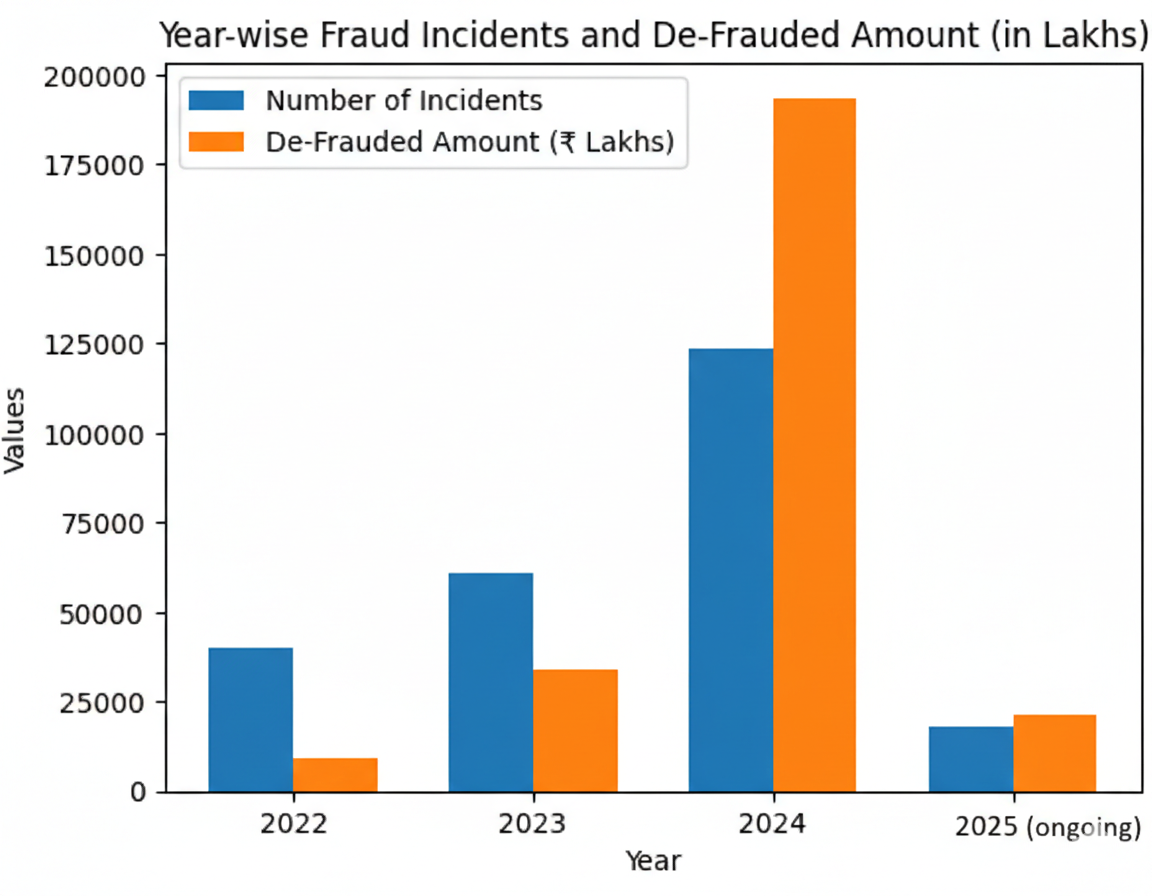
\includegraphics[width=\linewidth]{graph.png}
\end{column}

\end{columns}

% ---------- Rest of the slide (UNCHANGED, full width) ----------
\textbf{Social Impacts}
\begin{itemize}
  \item Loss of trust in digital governance and law enforcement institutions
  \item Elderly citizens and non-technical users become primary targets
  \item The gap in digitalization of rural and urban communities increases
\end{itemize}

\vspace{0.2cm}

\textbf{Economic Impacts}
\begin{itemize}
  \item Reduced public confidence in digital payment ecosystems
  \item Use of foreign accounts by scammers lead to loss of national capital
  \item Loss of long-term life savings by households
\end{itemize}

\end{frame}



% Slide 3: Future Scope and Mitigation
\begin{frame}{Mitigation Techniques}

\textbf{Individual-Level Mitigation}
\begin{itemize}
  \item Never trust arrest threats made via phone or video calls
  \item Do not share OTPs, Aadhaar, PAN, or bank details
\end{itemize}

\vspace{0.3cm}

\textbf{Institutional and Technological Solutions}
\begin{itemize}
  \item AI-based scam call and fraud detection systems
  \item Stronger KYC norms and real-time transaction monitoring
  \item Rapid-response cybercrime helplines and reporting mechanisms
  \item Integration of real-time fraud alerts in banking applications
\end{itemize}

\vspace{0.3cm}

\textbf{Future Scope}
\begin{itemize}
  \item Nationwide digital literacy and awareness campaigns
  \item Stronger cyber laws and international cooperation
\end{itemize}

\end{frame}

% Thank You Slide
\begin{frame}{Thank You}

\centering
\vspace{0.3cm}

{\Huge \textbf{Thank You}}

\vspace{0.6cm}

\small
\textbf{References}

\vspace{0.2cm}

\begin{itemize}

  \item \href{https://www.thehindu.com/news/national/digital-arrest-scam-how-to-protect-yourself/article68806494.ece}
  {The Hindu Bureau. “What Is ‘Digital Arrest Scam’ and How Can You Protect Yourself?” 
  \textit{The Hindu}, Oct. 2024.}

  \item \href{https://www.niti.gov.in/sites/default/files/2025-04/Digital_Arrest_The_Modern_Day_Cyber_Scam.pdf}
  {Singh, Major Sadhana. “Digital Arrest: The Modern Day Cyberscam.” 
  \textit{NITI Aayog}, Nov. 2025.}

  \item \href{https://www.data.gov.in/resource/year-wise-number-incidents-digital-arrest-scams-and-related-cyber-crimes-reported-national}
  {“Year-wise Number of Incidents of Digital Arrest Scams and Related Cyber Crimes Reported on National Cyber Crime Reporting Portal from 2022 to 2025.” 
  \textit{Open Government Data Platform India}, 30 May 2025.}

\end{itemize}

\end{frame}

\end{document}
